\begin{frame}{Base de dados - FER2013}
    
\begin{columns}
    \begin{column}{0.5\textwidth}
      \begin{itemize}
            \item 35887 amostras
            \item 48 x 48, grayscale
            \item $\pm$ centralizada
            \item $\approx$ igualmente distribuída
            \item Sete categorias
                \begin{itemize}
                    \item 0 - Raiva
                    \item 1 - Nojo
                    \item 2 - Medo
                    \item 3 - Felicidade
                    \item 4 - Tristeza
                    \item 5 - Surpresa
                    \item 6 - Neutro
                \end{itemize}
        \end{itemize}
    \end{column}
    
    \begin{column}{0.6\textwidth}
          \begin{figure}
            \centering
            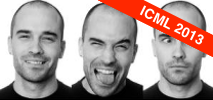
\includegraphics[width=0.7\linewidth]{img/front_page.png}
            \caption{Facial Expression Recognition Challenge \cite{carrier_courville}.}
          \end{figure}
    \end{column}
    
\end{columns} 
    
\end{frame}

\begin{frame}{Base de dados - Distribuições de expressões}

\begin{figure}
    \centering
    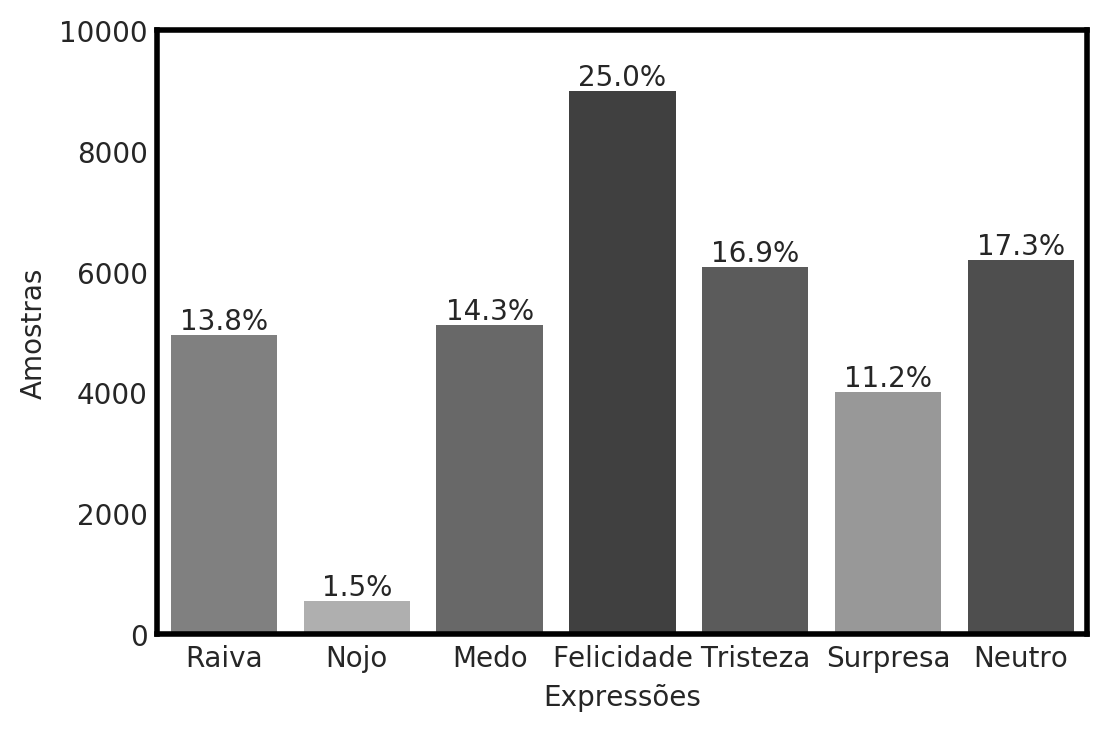
\includegraphics[width=0.9\linewidth]{img/expression_distribution.png}
    \caption{Distribuição de imagens por tipo de expressão facial FER2013.}
\end{figure}

\end{frame}

\begin{frame}{Base de dados - Distribuição de amostras}
    
\begin{figure}[h!]

	\begin{tabular}{@{}c@{}}
		\subfloat[Treinamento]{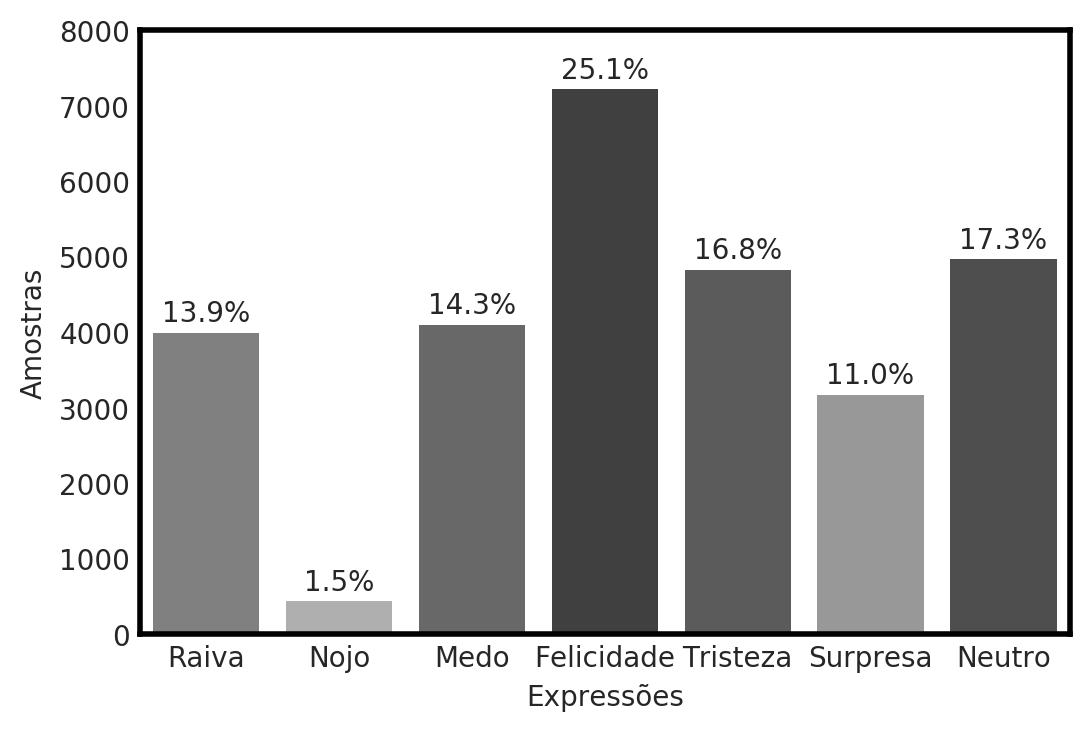
\includegraphics[width=0.4\linewidth]{img/expression_distribution_training.png}}
	\subfloat[Validação]{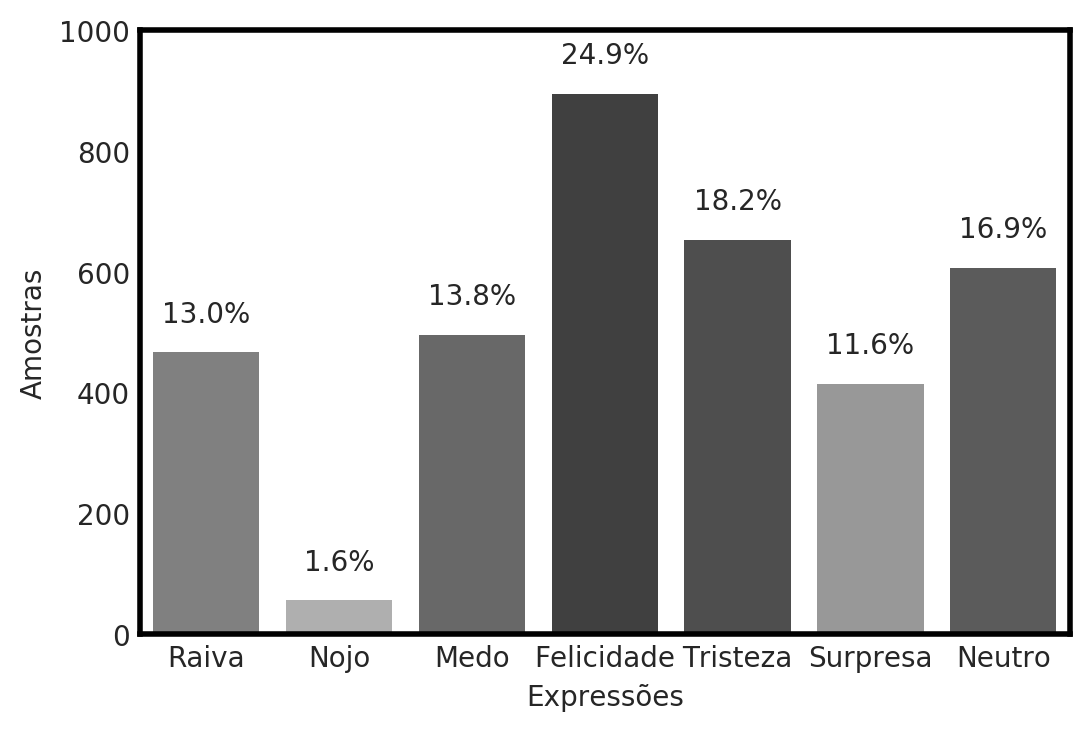
\includegraphics[width=0.4\linewidth]{img/expression_distribution_validation.png}}
	\end{tabular}

  \begin{tabular}{@{}c@{}}
		\subfloat[Teste]{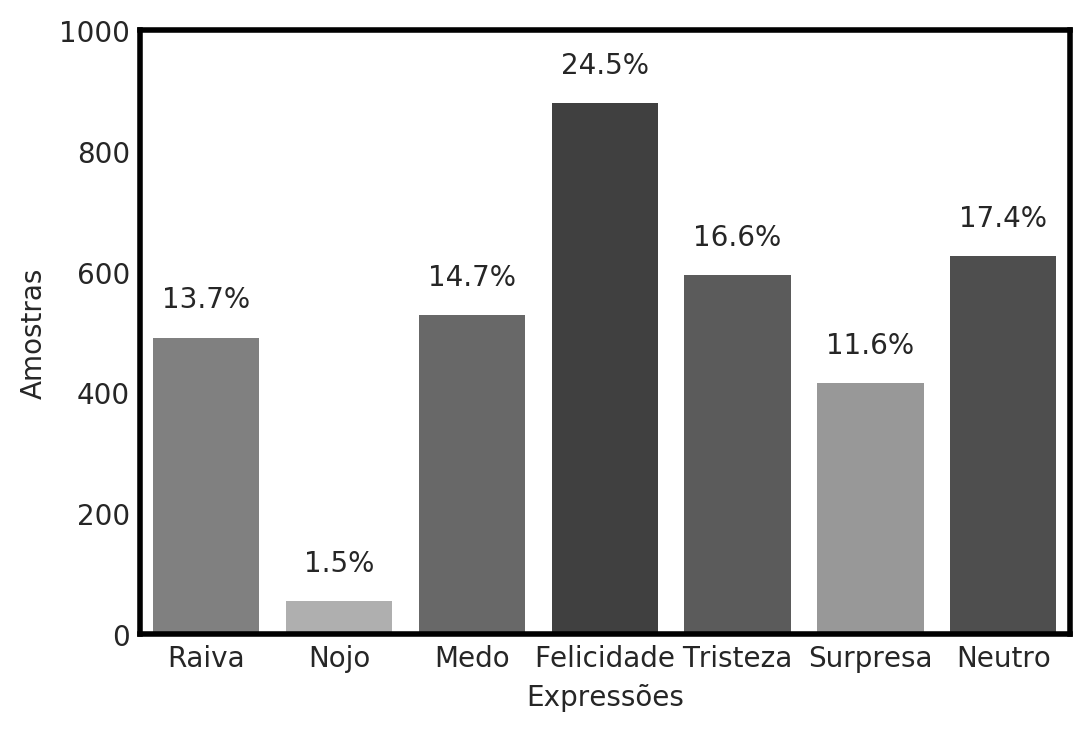
\includegraphics[width=0.4\linewidth]{img/expression_distribution_test.png}}
  \end{tabular}
  \caption{Distribuição de classes em cada partição.}
\end{figure}
    
\end{frame}